\documentclass{article}

\usepackage[margin=2cm]{geometry}
\usepackage{graphicx}
\usepackage{graphics}
\usepackage{hyperref}
\usepackage{psfrag}
\usepackage{ifthen}
\usepackage{array}
\usepackage{longtable}
\usepackage{color}
\usepackage{tikz}
\usepackage{amsmath, amsfonts, amsthm}
\usepackage[shortlabels]{enumitem}
\setcounter{secnumdepth}{0}
\newcommand{\N}{\mathbb{N}}
\newcommand{\R}{\mathbb{R}}


\begin{document}

\title{Homework 3}
\author{Hayden Pott}
\date{3 April 2024}

\maketitle

\section{1-60}
Determine which of the following statements are valid or invalid.
\begin{enumerate}[a)]

    \item I do well on the interview (I) and if my qualifications match the
        needs of the company (M), then I will get the job (J).  If I sleep
        the night before (S), I will do well on my interview. I slept well
        the night before and my qualifications match the needs of the
        company.  Therefore, I will get the job. \\
        \begin{align*}
            [[I \land M \implies J] \land 
            [S \implies I] \land 
            S \land M] \implies J
        \end{align*}
        \begin{center}
            \begin{tabular}{ |c|c|c|c|c|c|c|c|c| }
                \hline
                $J$ & $S$ & $I$ & $M$ & $I \land M$ & $I \land M \implies J$ & $S \implies I$ & $[I \land M \implies J] \land [S \implies I] \land S \land M$ & $H \implies J$ \\
                \hline
                %   J   S   I   M
                F & F & F & F & F & T & T & F & T \\
                F & F & F & T & F & T & T & F & T \\
                F & F & T & F & F & T & T & F & T \\
                F & F & T & T & T & F & T & F & T \\
                F & T & F & F & F & T & F & F & T \\
                F & T & F & T & F & T & F & F & T \\
                F & T & T & F & F & T & T & F & T \\
                F & T & T & T & T & F & T & F & T \\

                T & F & F & F & F & T & T & F & T \\
                T & F & F & T & F & T & T & F & T \\
                T & F & T & F & F & T & T & F & T \\
                T & F & T & T & T & T & T & F & T \\
                T & T & F & F & F & T & F & F & T \\
                T & T & F & T & F & T & F & F & T \\
                T & T & T & F & F & T & T & F & T \\
                T & T & T & T & T & T & T & T & T \\
                \hline
            \end{tabular}

        \end{center}
        \textbf{ANSWER:} Argument is valid.
\end{enumerate}

\newpage

\section{1-62}
Each of the following arguments involve qualified statements.  Determine which
\textit{arguments} are valid and which are not.
\begin{enumerate}[a)]
    \item Some mathematicians are brilliant.  Some brilliant people go crazy.
        Therefore, some mathematicians go crazy. \\
        \textbf{ANSWER:} Argument is invalid because of the instance where the
        mathematicians that are brilliant are \textit{not} the brilliant people
        that go crazy.  This is a counter-example to the statement that some
        mathematicians go crazy, thus the argument is invalid.
        (represented by the Venn diagram below)\\
        \begin{center}
            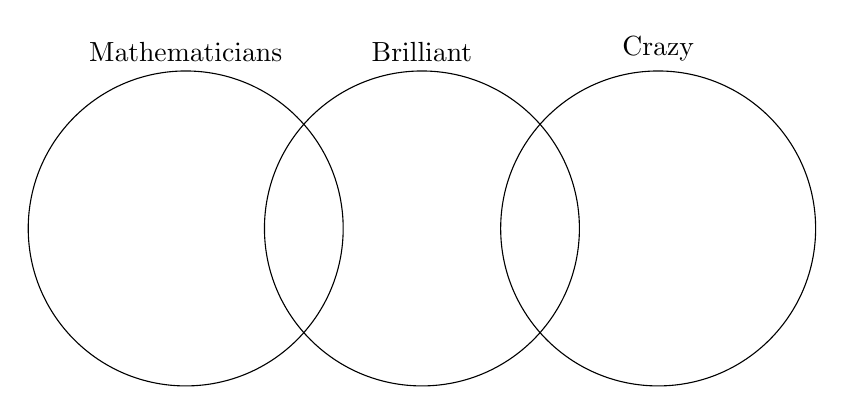
\begin{tikzpicture}
                \draw (0,0) circle (2) (0,2) node[text=black,above] {Mathematicians}
                (3,0) circle (2) (3,2) node[text=black,above] {Brilliant}
                (6,0) circle (2) (6,2) node[text=black,above] {Crazy};
            \end{tikzpicture}
        \end{center}
\end{enumerate}

\section{1-64}
Consider a database that catalogue other databases.  Prove that there cannot be
a database that lists all databases that do not list themselves. \\
\textbf{ANSWER:}
\begin{proof}
    SFAC that assumptions 1-3 can be satisfied. For a given $x$ the sentence
    $p(x) =$ ``x is a database'' $\land x \not\in x$ is an open sentence. Thus,
    assumption 3 guarantees that we can form the database $L = \{ D : p(D) \}$
    which lists all databases that do not list themselves. \\

    Now we consider if the set $L$ is an element of itself.  The statement $L
    \not\in L$ is either true or false. SFAC that $L \not\in L$ is true.  Then
    $L$ is not an element of itself.  By definition of $L$ being all databases
    which do not list themselves, we must conclude that $L$ is an element of
    itself. Contradiction.  Thus, $L \not\in L$ \textit{must} be false. \\

    But then, $L$ is an element of itself which means that $L$ does not satisfy
    the condition $A \not\in A$ used to define $L$.  This in turn implies that
    $L$ is not an element of itself.  Contradiction. \\

    Thus, $L$ can \textit{not} exist because its very existence is a
    contradiction.
\end{proof}
\begin{align*}
    L = \{D : D\text{ is a database} \land D \not\in D\}
\end{align*}
\end{document}
